
\chapter{Synchronous Machine Simulation}\label{chap:syncmach}

The purpose of this chapter is to assess the performance of the QDL method to the time-domain simulation of a highly non-linear, complex component of power systems: a three-phase synchronous generator.

In chapter \ref{chap:examples}, a dense, linear network having a very high stiffness ratio ($10^9$) was simulated using a combination of LIQSS1 and latency methods \cite{schutt2001}. The QDL method successfully solved the system response when conventional methods could not (or would have required impractically long simulation times). That work did not address the implications of non-linear system elements. In the previous works surveyed that use QSS integration, the feasibility and performance of QSS-based methods were investigated only for linear systems or for very small non-linear systems (In Di Pietro et al., \cite{pietro2018} for example, a four-stage interleaved converter was simulated using QSS). This chapter attempts to take this a step further by simulating a higher order non-linear power system, specifically with detailed synchronous machine model. 

Systems that include synchronous machines often operate for a long duration in mostly steady-state conditions. These steady conditions are occasionally punctuated by abrupt changes of conditions that must be accurately simulated. The QDL method has the potential for high computational efficiency for simulation of such systems. Non-linearity, high stiffness, and a necessity for algebraic constraints to enforce circuit conservation laws are the important aspects of these systems that we feel QDL is well-suited for.

\section{Study System}

\begin{figure}[h]
    \centering
    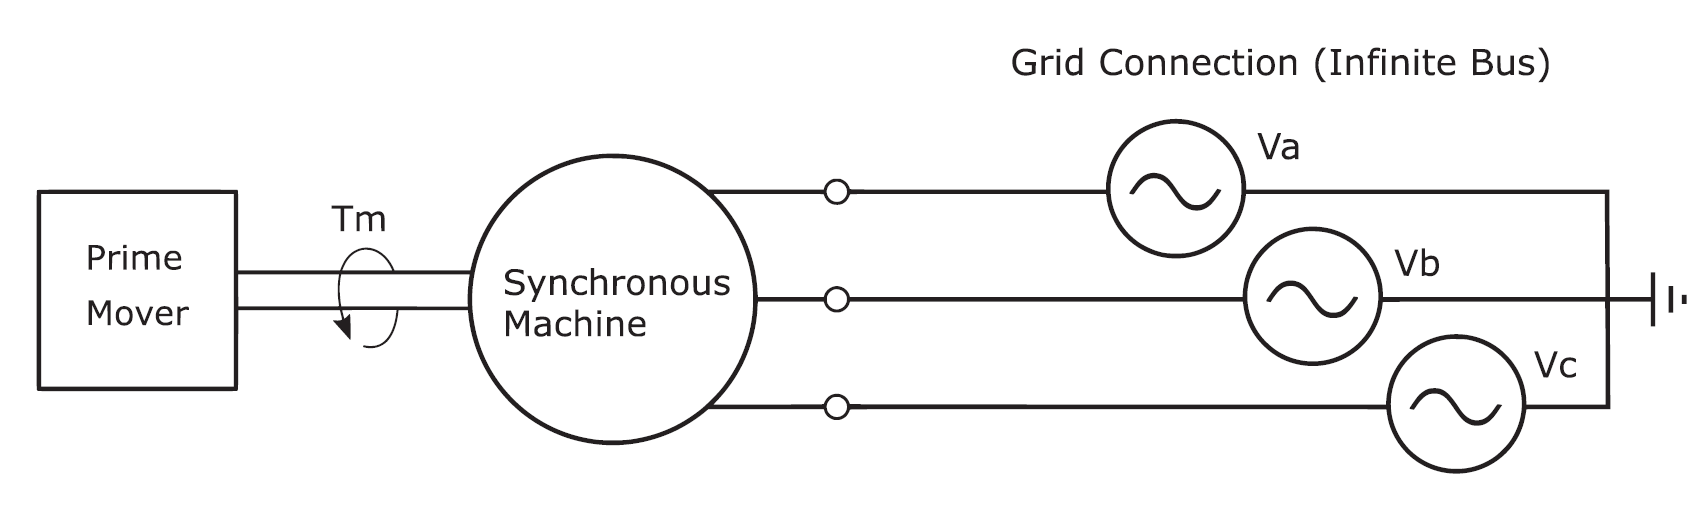
\includegraphics[width=0.8\linewidth]{syncmach_schem.png}
    \caption{Synchronous generator connected to an infinite bus.}
    \label{fig:syncmach_schem}
\end{figure}

The study system, shown in figure \ref{fig:syncmach_schem}, has three major components: a prime mover, a synchronous machine (which can act as either a generator or a motor depending on the direction of power flow), and an simple ac power grid model. Models of the prime mover and the grid are simplified. The torque source is an ideal time-dependent source with zero inertia, and the power system is represented as an ideal three-phase sinusoidal ac voltage source with zero impedance and constant frequency (i.e. an infinite bus). This study system was chosen because it is of widespread interest in power systems analysis (the so-called single machine infinite bus, or SMIB system), and because it demonstrates suitability of the QDL method to efficiently solve non-linear systems that are characterized by coupled fast and slow dynamics.

\section{Synchronous Machine Model}

The model of the electric machine is formulated in the synchronous reference frame to eliminate the periodic sinusoidal variations of all voltages and currents via the standard Park transformation \cite{andanapalli2014}. This maximizes the benefit of using the QDL method for the analysis of ac systems, as the potential for slower updates during steady-state conditions relies on flat (zero-derivative) states in steady-state. Although QDL can be used to simulate systems having arbitrary wave forms, the sinusoidal voltage and current oscillations inherent in an ac power system would require rapid state updates that would negate any benefits offered by the QDL method.

\begin{figure}[h]
    \centering
    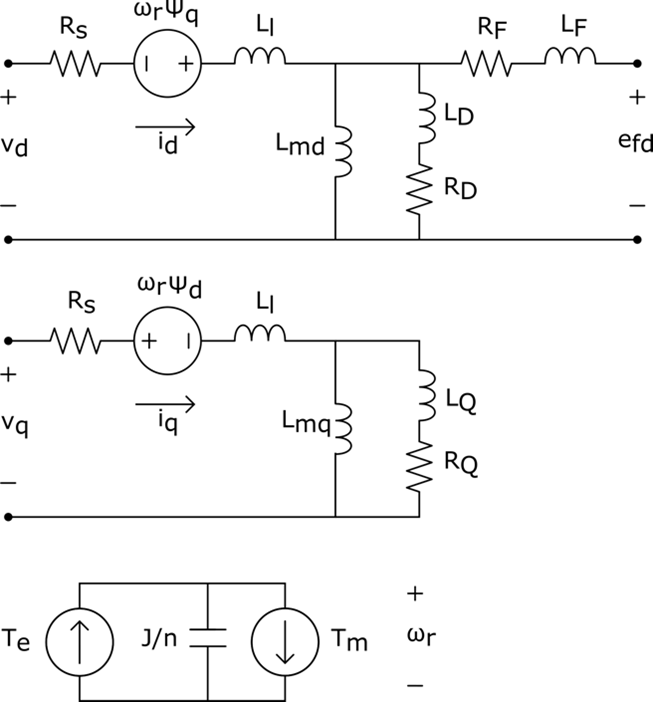
\includegraphics[width=0.8\linewidth]{syncmach_circuit.png}
    \caption{Direct, quadrature, and mechanical equivalent
        circuits of the synchronous machine.}
    \label{fig:syncmach_circuit}
\end{figure}

A common model of the synchronous generator formulated in the synchronous reference frame is described by the set of equivalent circuits shown in figure \ref{fig:syncmach_circuit}. The fundamental frequency of the study system is 50 Hz. The seventh-order set of nonlinear equations that describe the dynamics of the transformed circuit is described in Equations \ref{eq:sync_mach_diffeq_1} through \ref{eq:sync_mach_diffeq_7}, and the algebraic constraints that apply to the network solution are defined by Equations \ref{eq:sync_mach_alg_1} and \ref{eq:sync_mach_alg_2}. Figure \ref{fig:syncmach_circuit} and the equations follow the model described in \cite{ieee1110}.

\begin{equation}
    \label{eq:sync_mach_diffeq_1}
    \frac{d}{dt} \psi_d = v_d - R_s i_d + \omega_r \psi_q
\end{equation}

\begin{equation}
    \label{eq:sync_mach_diffeq_2}
    \frac{d}{dt} \psi_q = v_q - R_s i_q - \omega_r \psi_d
\end{equation}

\begin{equation}
    \label{eq:sync_mach_diffeq_3}
    \frac{d}{dt} \psi_F = e_{fd} - i_F R_F
\end{equation}

\begin{equation}
    \label{eq:sync_mach_diffeq_4}
    \frac{d}{dt} \psi_D = -i_D R_D
\end{equation}

\begin{equation}
    \label{eq:sync_mach_diffeq_5}
    \frac{d}{dt} \psi_Q = -i_Q R_Q
\end{equation}

\begin{equation}
    \label{eq:sync_mach_diffeq_6}
    \frac{d}{dt} \omega_r = \frac{n}{J} (i_q \psi_d - i_d \psi_q - T_m )
\end{equation}

\begin{equation}
    \label{eq:sync_mach_diffeq_7}
    \frac{d}{dt} \theta = \omega_r - \omega_b
\end{equation}

\begin{equation}
    \label{eq:sync_mach_alg_1}
    \begin{bmatrix}
        i_{dr} \\
        i_F    \\
        i_D
    \end{bmatrix}
    =
    \begin{bmatrix}
        L_{md} + L_{L} & L_{md}         & L_{md}         \\
        L_{md}         & L_{F} + L_{md} & L_{md}         \\
        L_{md}         & L_{F} + L_{md} & L_{F} + L_{md} \\
    \end{bmatrix}^{-1}
    \cdot
    \begin{bmatrix}
        \psi_{dr} \\
        \psi_F    \\
        \psi_D
    \end{bmatrix}
\end{equation}

\begin{equation}
    \label{eq:sync_mach_alg_2}
    \begin{bmatrix}
        i_{qr} \\
        i_Q  
    \end{bmatrix}
    =
    \begin{bmatrix}
        L_{mq} + L_{L} & L_{mq} \\
        L_{mq}         & L_{mq} \\
    \end{bmatrix}^{-1}
    \cdot
    \begin{bmatrix}
        \psi_q \\
        \psi_Q  
    \end{bmatrix}
\end{equation}

Where the terms in these equations are defined as:

\begin{align*}
    \psi_d   & \text{ : direct-axis and stator flux (Wb)}, \\
    \psi_q   & \text{ : quadrature-axis stator flux (Wb)}, \\
    \psi_D   & \text{ : direct-axis damper flux (Wb)}, \\
    \psi_Q   & \text{ : quadrature-axis damper flux (Wb)}, \\
    v_d      & \text{ : direct-axis terminal voltage (V)}, \\
    v_q      & \text{ : quadrature-axis terminal voltage (V)}, \\
    R_s      & \text{ : stator series resistance (} \Omega \text{)}, \\
    \omega_r & \text{ : rotor speed (rad/s)}, \\
    \omega_b & \text{ : base frequency (} 2 \pi 50 \text{ rad/s)}, \\
    i_d      & \text{ : direct-axis stator current (A)}, \\
    i_q      & \text{ : quadrature-axis stator current (A)}, \\
    \psi_F   & \text{ : stator field flux (Wb)}, \\
    i_F      & \text{ : stator field current (A)}, \\
    e_{fd}   & \text{ : field voltage (V)}, \\
    R_F      & \text{ : field resistance (} \Omega \text{)}, \\
    i_D      & \text{ : direct-axis internal equivalent current (A)}, \\
    i_Q      & \text{ : quadrature-axis internal equivalent current (A)}, \\
    R_D      & \text{ : direct-axis equivalent circuit resistance (} \Omega \text{)}, \\
    R_Q      & \text{ : quadrature-axis equivalent circuit resistance (} \Omega \text{)}, \\
    i_{dr}   & \text{ : direct-axis rotor current (A)}, \\
    i_{qr}   & \text{ : quadrature-axis rotor current (A), and}  \\
    \theta   & \text{ : rotor angle relative to synchronous reference frame  (rad).}
\end{align*}


\section{Simulation Scenario and Reference Solution}

The scenario is a typical simulation that initializes the system to steady-state at a specific operating point, and then adds a perturbation to produce a transient response. The simulation starts with the synchronous generator rotating at steady-state in synchronism with the connected grid. This steady-state condition continues for the first $15$ seconds. Beginning at time {t = 15s}, the torque applied by the prime mover to the shaft of the machine begins to ramp up. The torque ramp continues until time {t = 20s}, at which time the torque has reached $25\%$ of the machine’s rated torque. At $25\%$ of rated torque, the phase of the stator voltage leads that of the grid voltage, and the machine drives about $83 MW$ active power and $13 MVAr$ reactive power into the grid.

The system was first simulated using a reference (benchmark) simulation to provide a basis for performance and accuracy comparison of the QDL simulation. The reference solution was obtained by using an implicit Euler integration in MATLAB. A fixed time step of ($10^{-4} s$) was chosen for the Euler solution to ensure stability considering the entire range of eigenvalues. The QDL simulation was obtained by using the LIQSS1 integration method described below.

\section{Implementation of the QDL Model}

The specific QSS integration method used for this example is LIQSS1, described in \cite{pietro2018} and \cite{migoni2009}. The system model comprises seven QDL atom models, one for each of the seven state variables. Figure \ref{fig:syncmach_connect} shows the seven QDL atoms comprising the synchronous machine with directional arrows indicating the external transition graph connections. The system is tightly coupled and components have bidirectional connections. Bi-directional arrows indicate that a state update of either atom requires an update of the other. As an example, following the string of just one arrow, any update to the output of $\psi_{dr}$ requires $\omega_r$ to update the time at which it expects to reach its next quantum level. If the update of $\psi_{dr}$ results in a change of the quantized state of $\omega_r$, then the $\theta$ atom will update the estimate of its transition time to the next quantum transition, and that will feed back to require a next update of $\psi_{dr}$.

To start the solution, the next update time of each atom is initialized to infinity. Each atom then independently computes its own next update time (the time at which it should arrive at its next higher or lower quantum state). The atom with the nearest update time is then updates its external state ($q$) to the appropriate adjacent quantum level. This external state update then flags the connected atoms to update their internal states and next external transition time, and the loop continues. A flowchart of the process is shown in chapter \ref{chap:qdl} figure \ref{fig:qdl_flowchart}.

\begin{figure}[h]
    \centering
    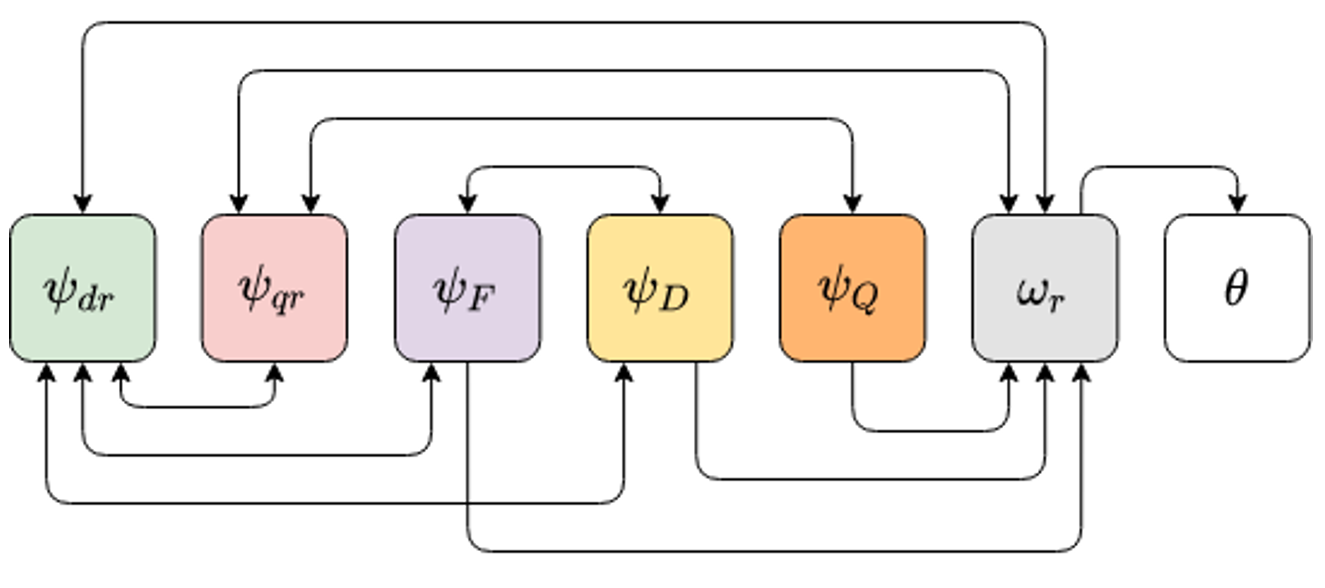
\includegraphics[width=0.8\linewidth]{syncmach_connect.png}
    \caption{Synchronous machine model QDL atoms showing the external state transition connections.}
    \label{fig:syncmach_connect}
\end{figure}

\section{QDL Performance}

The performance of the QDL method is shown in comparison to the performance of the reference solution in a series of plots. Each plot shows the trajectory of a state variable and the cumulative number of updates (or re-evaluations) of the QDL atom for that state variable. All states in the system use the same quantization step size ($\Delta Q$) of $10^{-4} Wb$, except the machine rotor speed ($\omega_r$) for which we choose a $\Delta Q$ $1/10^{th}$ as large as the others ($10^{-5} rad/s$) since the dynamic range of the rotor speed is much less than that of the system fluxes. For simplicity, this simulation does not use a complex methodology for choosing the best $\Delta Q$. A $\Delta Q$ of roughly 0.1\% of the total expected deviation (the absolute value of the dynamic range of the quantity in the reference simulation) of the quantized state variable. Another objective of the this simulation is to investigate the relationship between $\Delta Q$ and solution error. Understanding this relationship could lead to a more rigorous methodology for choosing $\Delta Q$ based on a desired error bound. Figures \ref{fig:syncmach_fdr}, \ref{fig:syncmach_fqr} and \ref{fig:syncmach_fF} show the accuracy with which the QDL method tracks the reference solution. The cumulative number of updates for a particular atom is shown by the red lines in the following charts, with each state's cumulative updates being unique. Further discussion on the relationship between $\Delta Q$ and error, and alternative methods for $\Delta Q$ selection can be found in chapter \ref{chap:deltaq}.

An performance advantage of the QDL method over the reference solution can be seen as the system reaches the new steady state condition and the rate of atom updates markedly decreases. For example, in figure \ref{fig:syncmach_fdr}, during the interval from 0 to 15 seconds, while the system is in steady-state, there are very few state updates. During the period from 15 sec to 35 seconds, however, while the machine is accelerating (and the other states of the system are rapidly changing), the slope of the curve representing the cumulative number of updates is large. Finally, after around 35 seconds, the system approaches a new steady-state and the update rate decreases. This aspect of the QDL method allows the simulation to advance rapidly during steady-state conditions, and speed up again when fast transient behavior requires more time resolution. Also, the cumulative number of updates depends on the chosen $\Delta Q$. In general, a smaller $\Delta Q$ will tend to require more frequent updates, and the simulation will tend to advance more slowly through time. However, it is important to note that the effects of changing the $\Delta Q$ on performance and accuracy is complex, and warrants further discussion and investigation (see chapter \ref{chap:deltaq}).

\begin{figure}[h]
    \centering
    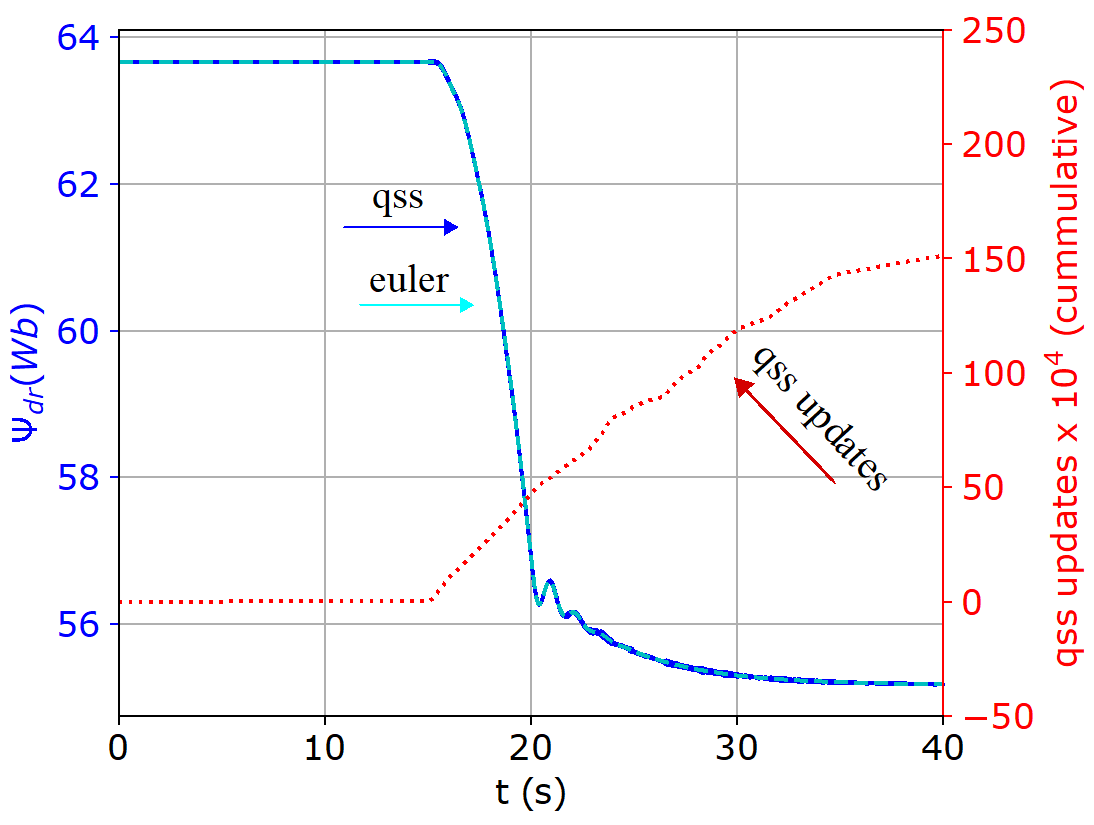
\includegraphics[width=0.8\linewidth]{syncmach_fdr.png}
    \caption{Rotor d-axis flux. The flux computed by the QDL method is nearly identical to that computed by the reference method so the two lines are nearly indistinguishable. Cumulative count of $\psi_{dr}$ atom updates shows little activity prior to torque ramp, higher activity during torque ramp, and a return to little activity as new steady state is attained.}
    \label{fig:syncmach_fdr}
\end{figure}

\begin{figure}[h]
    \centering
    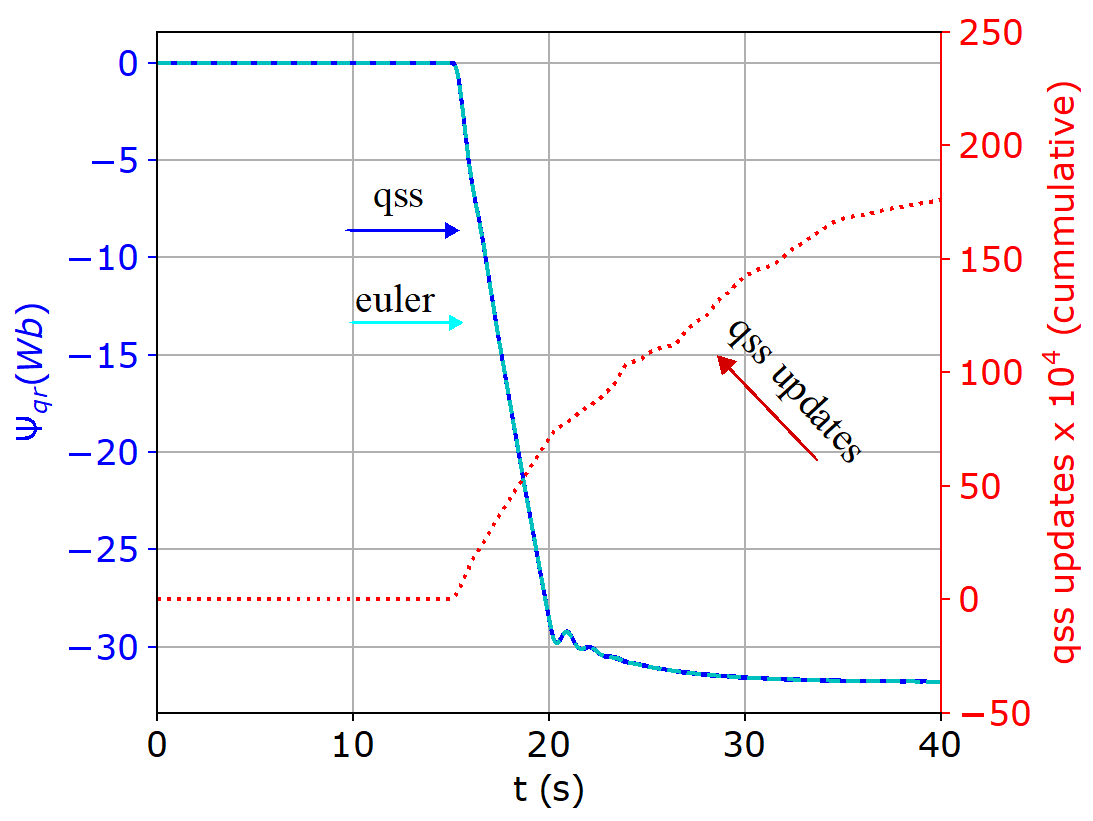
\includegraphics[width=0.8\linewidth]{syncmach_fqr.png}
    \caption{Rotor q-axis flux. The values computed by the QDL method and the reference method are nearly indistinguishable.}
    \label{fig:syncmach_fqr}
\end{figure}

\begin{figure}[h]
    \centering
    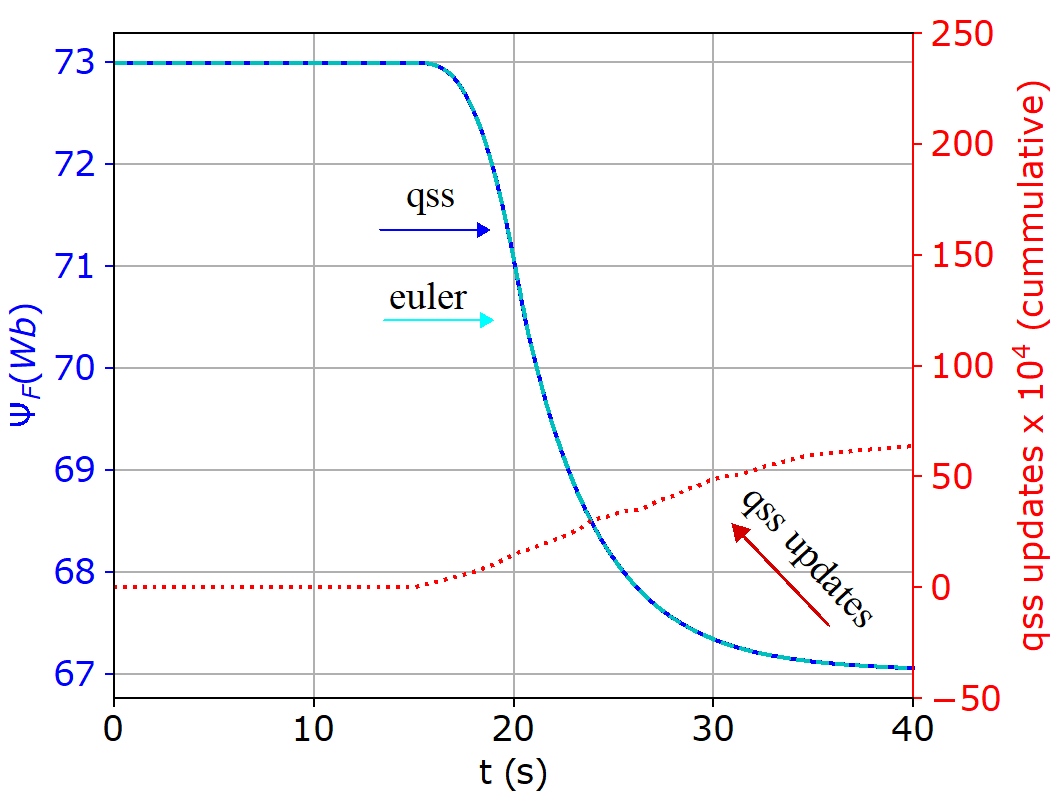
\includegraphics[width=0.8\linewidth]{syncmach_fF.png}
    \caption{Field flux, showing good agreement between both computing methods and a total number of QDL atom updates that is smaller than the counts for d- and q-axis fluxes.}
    \label{fig:syncmach_fF}
\end{figure}

\begin{figure}[h]
    \centering
    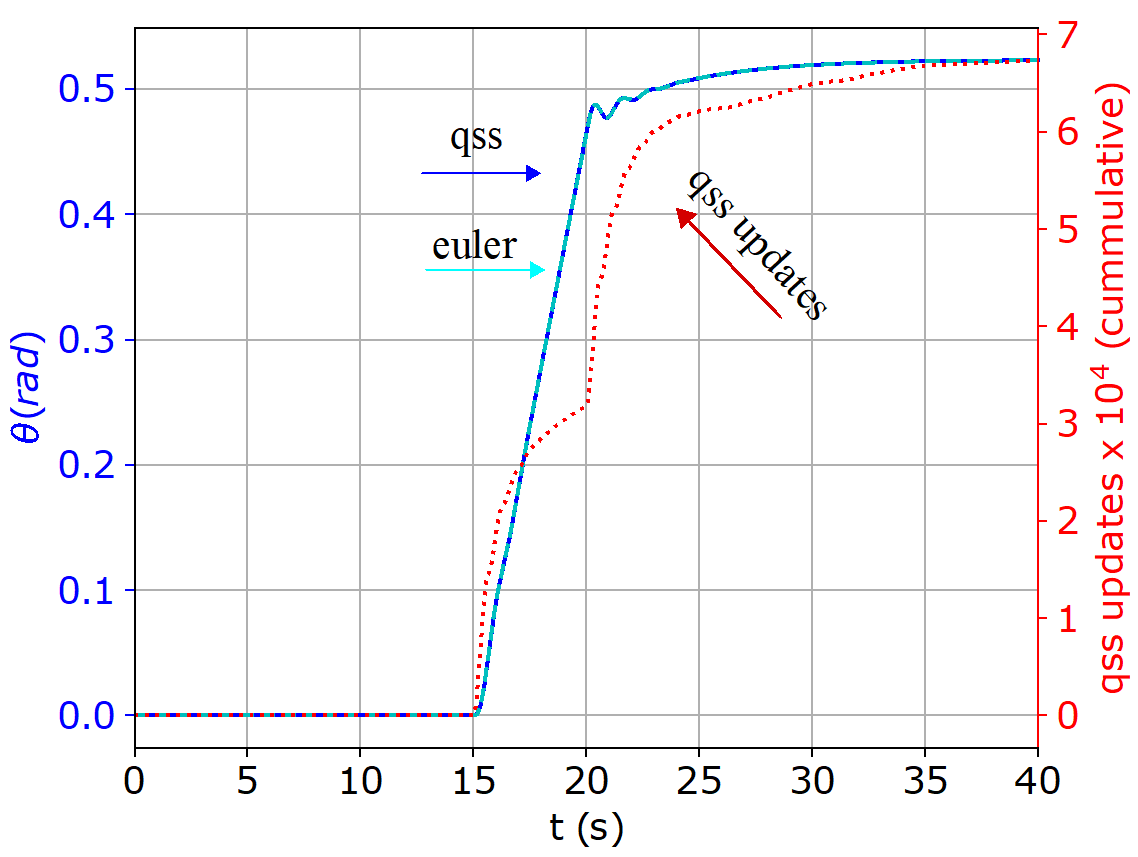
\includegraphics[width=0.8\linewidth]{syncmach_theta.png}
    \caption{Rotor angle. QDL update rate shows interesting behavior with faster rates associated with beginning and ending of the torque ramp.}
    \label{fig:syncmach_theta}
\end{figure}

The trajectory of rotor angle ($\theta$) , as shown in figure \ref{fig:syncmach_theta}, is particularly interesting in that it shows how the count of this atom’s updates increases immediately after the start of the torque ramp-up, then tapers off while the torque slew rate is constant during the interval between 15 to 20 seconds, then increases again at 20 seconds when the torque stops moving, and finally becomes small again as the rotor angle reaches its final steady state value. Figure \ref{fig:syncmach_wr} shows the trajectory of the rotor speed which always remains very close to 100 rad/s, but shows structure near the beginning and ending of the torque ramp, and a small speed increase during the torque ramp-up.

\begin{figure}[h]
    \centering
    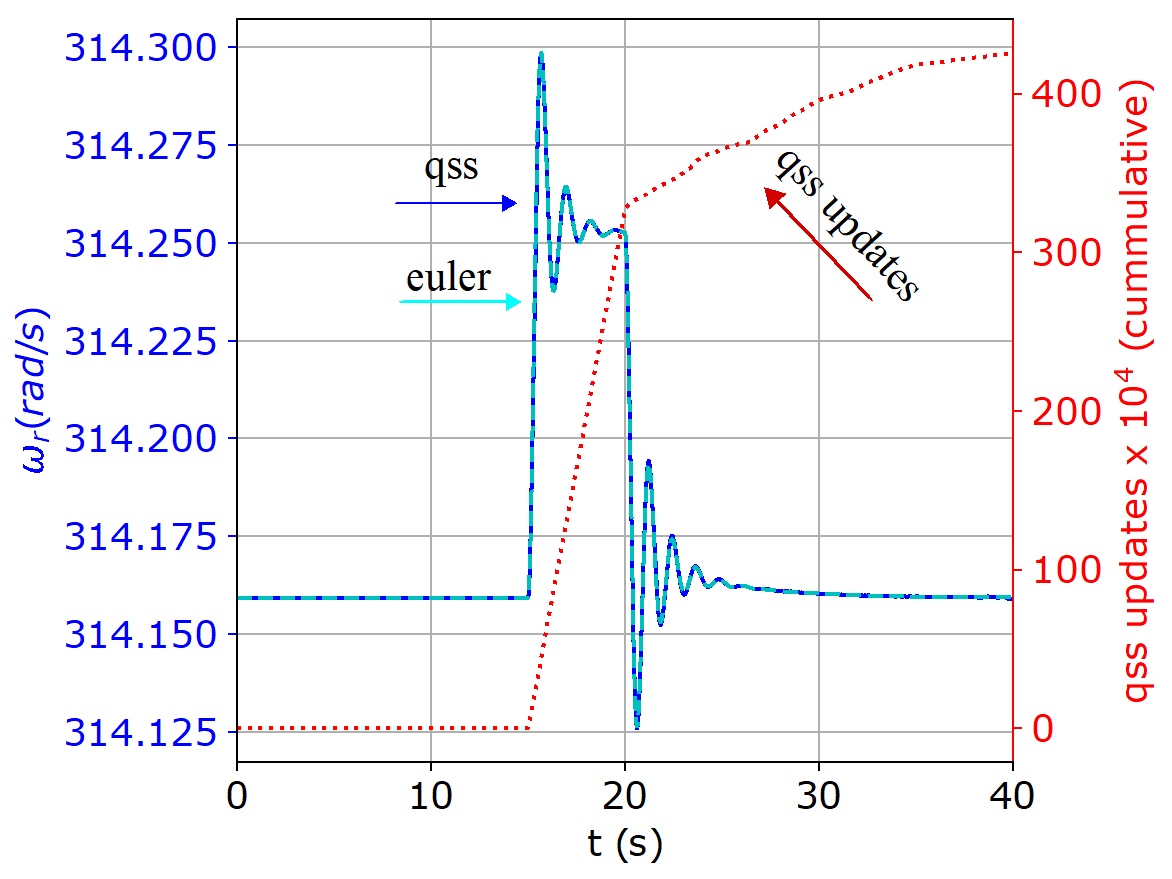
\includegraphics[width=0.8\linewidth]{syncmach_wr.png}
    \caption{Rotor speed trajectory and update rates.}
    \label{fig:syncmach_wr}
\end{figure}

\begin{figure}[h]
    \centering
    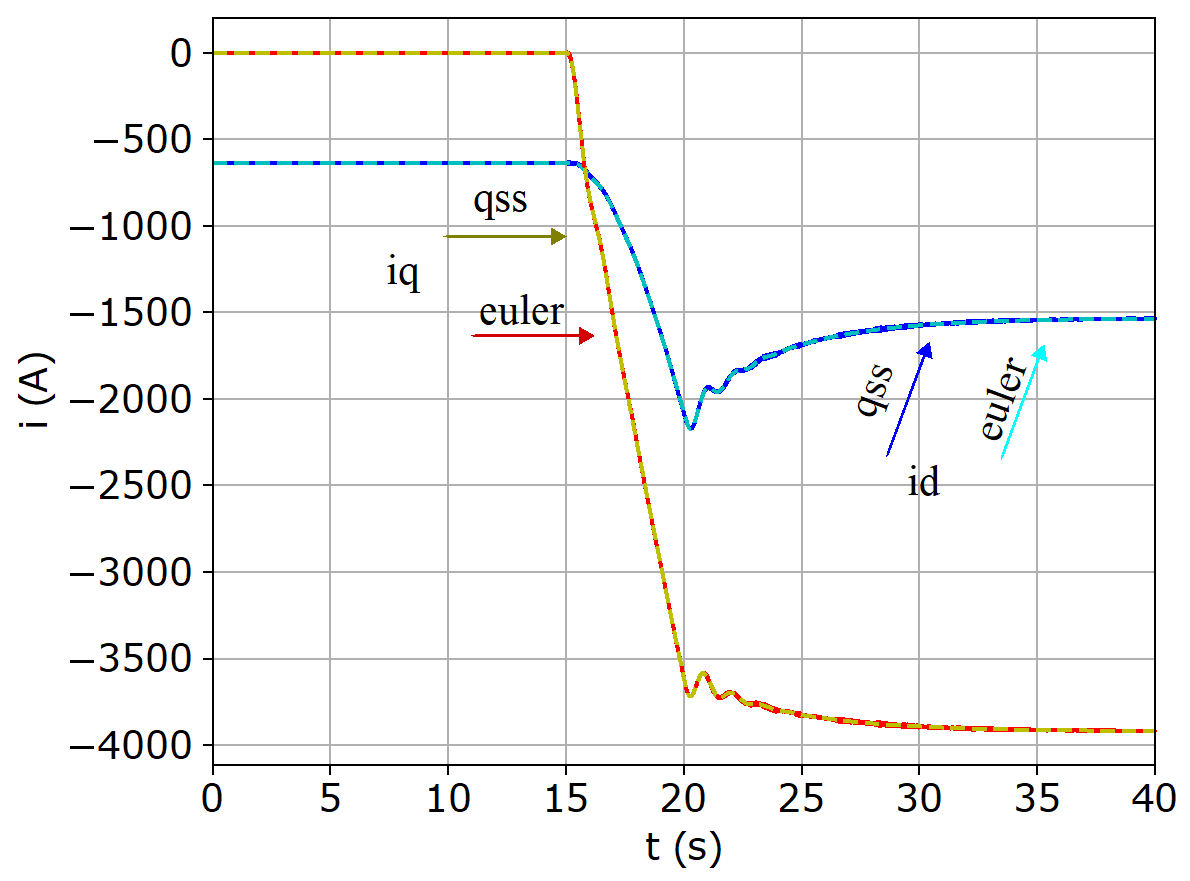
\includegraphics[width=0.8\linewidth]{syncmach_current.png}
    \caption{Comparisons of d- and q-axis rotor currents computed by the QDL and reference solutions.}
    \label{fig:syncmach_current}
\end{figure}

\begin{figure}[h]
    \centering
    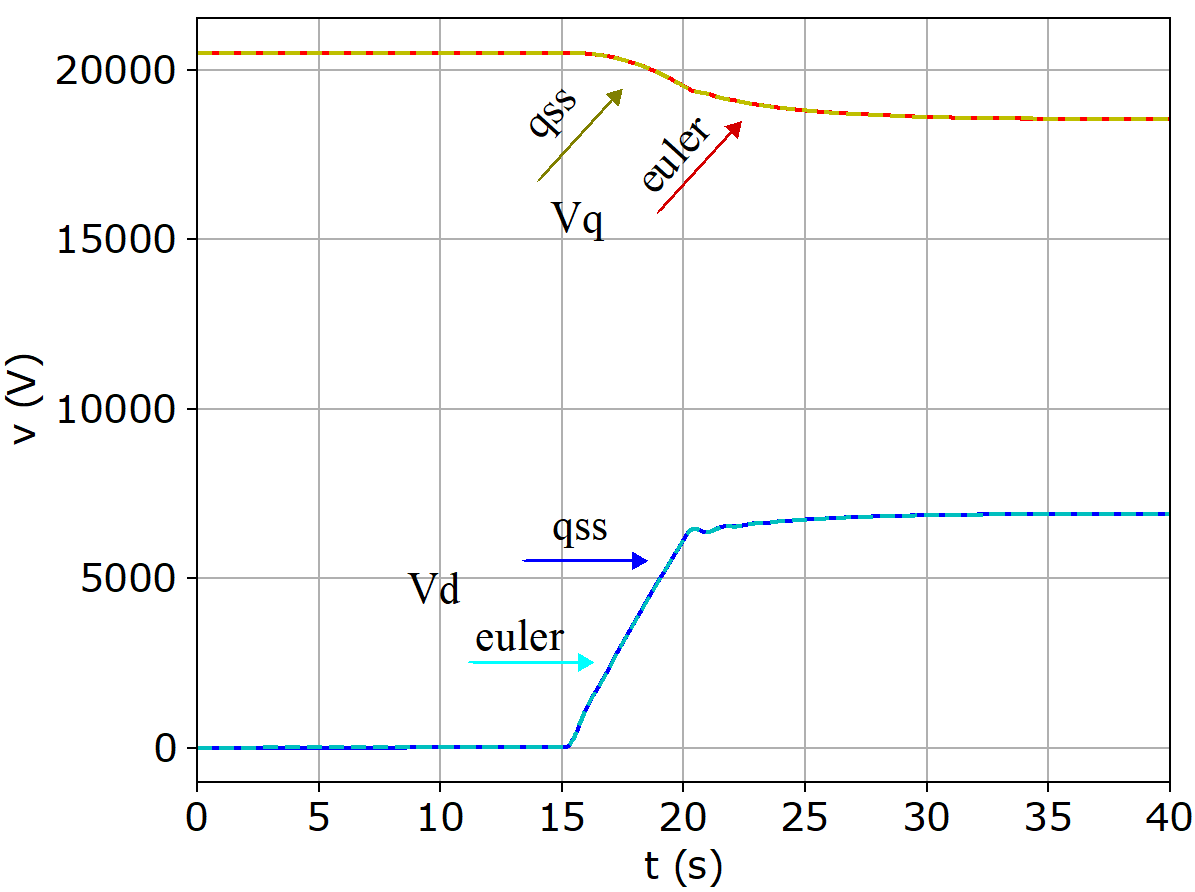
\includegraphics[width=0.8\linewidth]{syncmach_voltage.png}
    \caption{Comparisons of d- and q-axis voltages computed by the QDL and reference solutions.}
    \label{fig:syncmach_voltage}
\end{figure}

\section{Accuracy and Error Analysis}

In \cite{kofman2001b}, the authors proved that, for linear time-invariant systems, the global error in QSS integration solutions can be bounded by a constant proportional to the quantization step size ($\Delta Q$). However, our reference system is highly non-linear, so it is interesting to explore the behavior of error with varying $\Delta Q$. 
The effect $\Delta Q$ on simulation accuracy is shown in figures \ref{fig:syncmach_wr_qstep}, \ref{fig:syncmach_wr_qstep_ZOOM} and \ref{fig:syncmach_wr_qstep_ZOOM2}, where several system variables are plotted for a range of $\Delta Q$ values, with enhanced detail during particular time periods.  A larger quantization step  size results in both a lower update rate and a higher error amplitude compared to a situation with a smaller $\Delta Q$. In each case, the quoted $\Delta Q$ applies to all of the state variables except rotor speed, for which the quantization step is $1/10^{th}$ that of the other variables. In each plot, the trajectory with green color corresponds to the largest $\Delta Q$ of $10^{-3}$, while blue and red correspond to smaller sizes ($\Delta Q = 10^{-4}$  and $\Delta Q = 10^{-5}$ respectively). The rotor speed calculated with the largest $\Delta Q$ has the largest error in comparison to the reference solution. This is evident in both figure \ref{fig:syncmach_wr_qstep_ZOOM}, in which resolution is increased near the apex of the speed trajectory, and in figure \ref{fig:syncmach_wr_qstep_ZOOM2} where higher resolution shows a slightly oscillating speed trajectory after the torque ramp. These high frequency oscillations are inherent to the QDL method and the amplitude of these oscillations increases as the $\Delta Q$ increases. The sensitivity data provided in this chapter have been empirically determined from simulation of this specific system with specific component parameters. Although this empirical data does provide useful insight into the relationship between $\Delta Q$ and error, it does not solve the problem for the general case.

\begin{figure}[h]
    \centering
    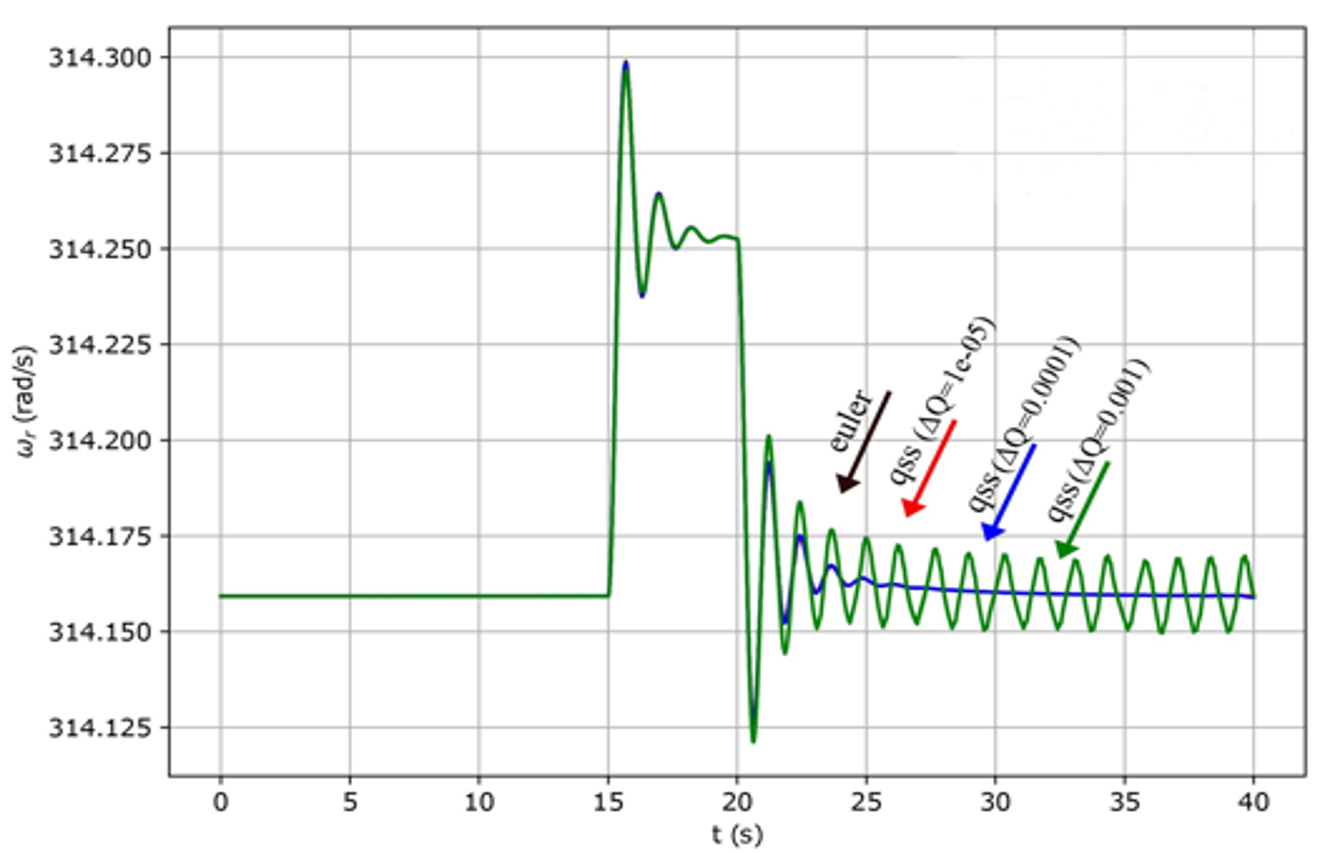
\includegraphics[width=0.8\linewidth]{syncmach_wr_qstep.png}
    \caption{Rotor speed using different quantization sizes ($\Delta Q = 10^{-5}$, $\Delta Q = 10^{-4}$, $\Delta Q = 10^{-5}$ vs Euler method reference solution.}
    \label{fig:syncmach_wr_qstep}
\end{figure}

\begin{figure}[h]
    \centering
    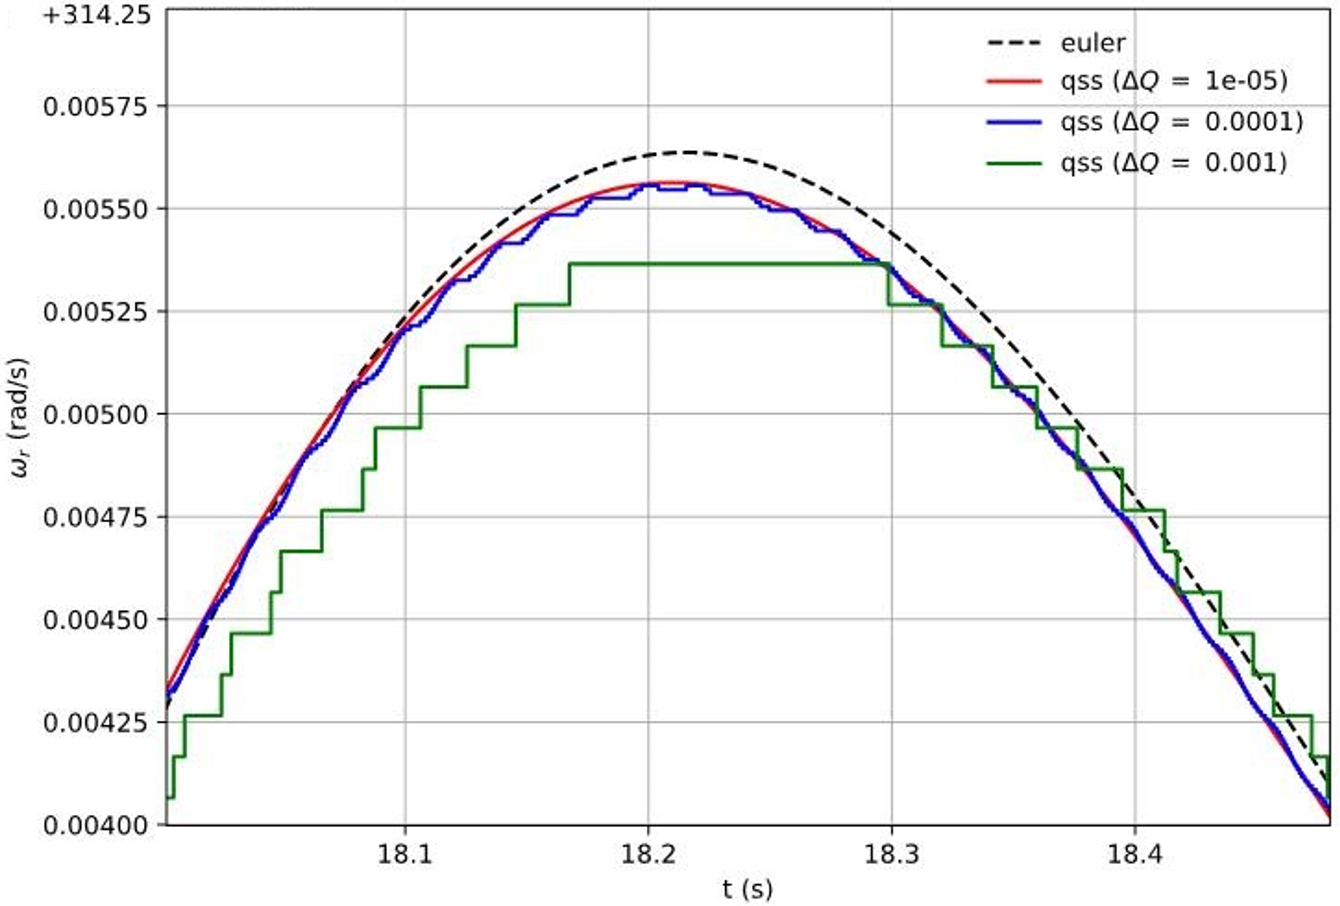
\includegraphics[width=0.8\linewidth]{syncmach_wr_qstep_ZOOM.png}
    \caption{Zoom plots from 18 sec to 18.5 sec of rotor speed using different quantization sizes $\Delta Q = 10^{-5}$, $\Delta Q = 10^{-4}$, $\Delta Q = 10^{-3}$ vs Euler method reference solution.}
    \label{fig:syncmach_wr_qstep_ZOOM}
\end{figure}

\begin{figure}[h]
    \centering
    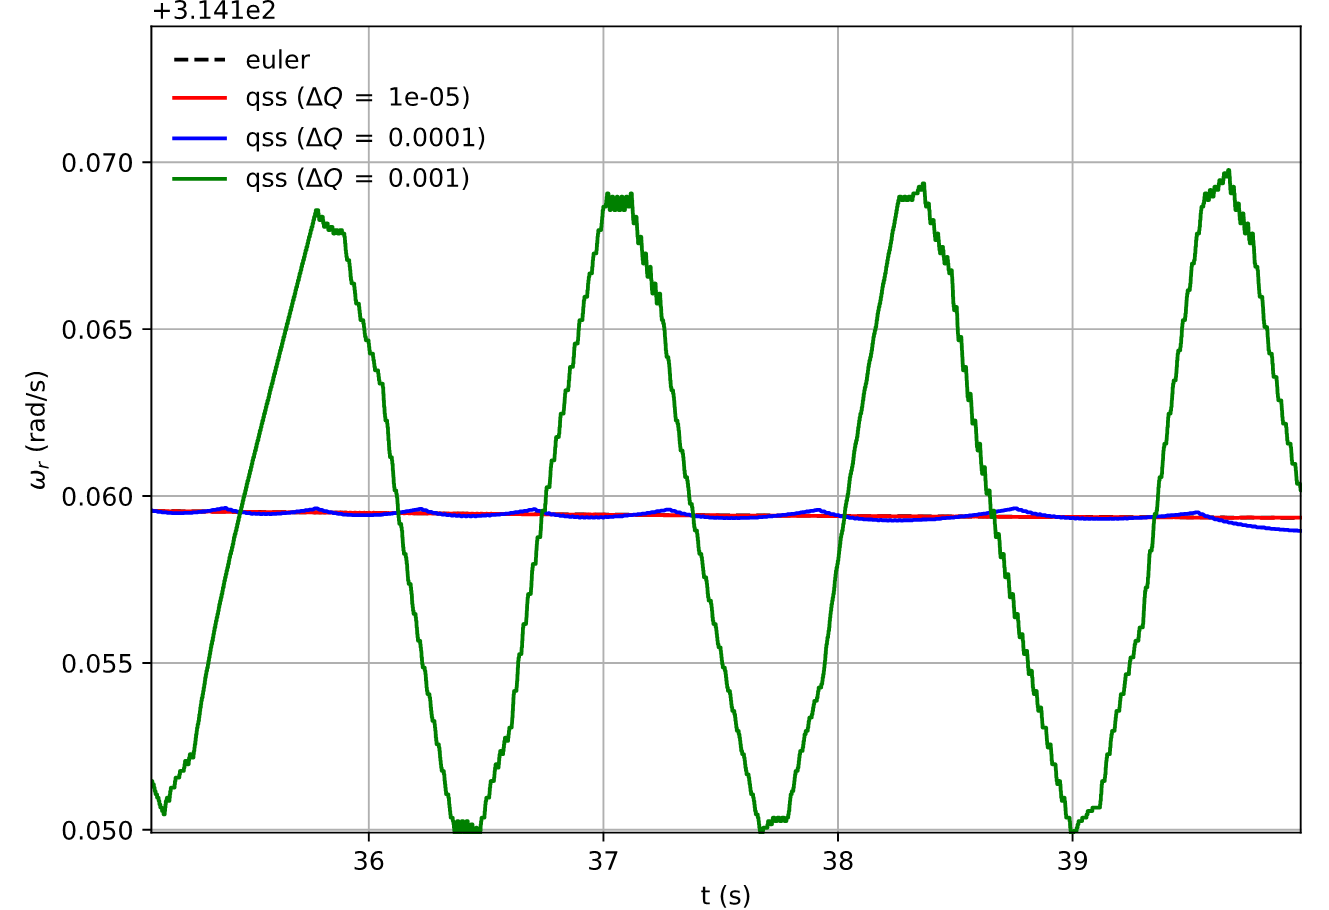
\includegraphics[width=0.8\linewidth]{syncmach_wr_qstep_ZOOM2.png}
    \caption{Zoom-in plots that show details for steady state situation of rotor speed using different quantization sizes $\Delta Q = 10^{-5}$, $\Delta Q = 10^{-4}$, $\Delta Q = 10^{-5}$ vs Euler reference solution. The oscillations have very small amplitudes.}
    \label{fig:syncmach_wr_qstep_ZOOM2}
\end{figure}

Figures \ref{fig:syncmach_wr_error_time} and \ref{fig:syncmach_wr_error_qstep} describe the same behavior as was shown in figures \ref{fig:syncmach_wr_qstep}, \ref{fig:syncmach_wr_qstep_ZOOM}, and \ref{fig:syncmach_wr_qstep_ZOOM2} but from the error perspective. Figure \ref{fig:syncmach_wr_error_time} shows how the point-wise absolute error (the difference between the QDL simulation and the reference simulation) varies over a particular half-second interval. The time variation of error in the state variable $\psi_{dr}$ is shown for several different $\Delta Q$ ranging from $\Delta Q = 10^{-6}$ to $\Delta Q = 10^{-2}$. Clearly, a larger $\Delta Q$ produces a larger error in this case, but the relationship was not linear. Before the torque ramps up, the different $\Delta Q$ values all produce negligible errors. After the torque starts to ramp up, the number of updates starts to grow and the models using larger quantization sizes produce larger errors. Although a small quantization size improves the simulation accuracy, it also causes a larger model update rate. Therefore, if computing speed is important, and if a larger percent error is tolerable, one might choose a large $\Delta Q$ in order to achieve the requisite computing speed.

\begin{figure}[h]
    \centering
    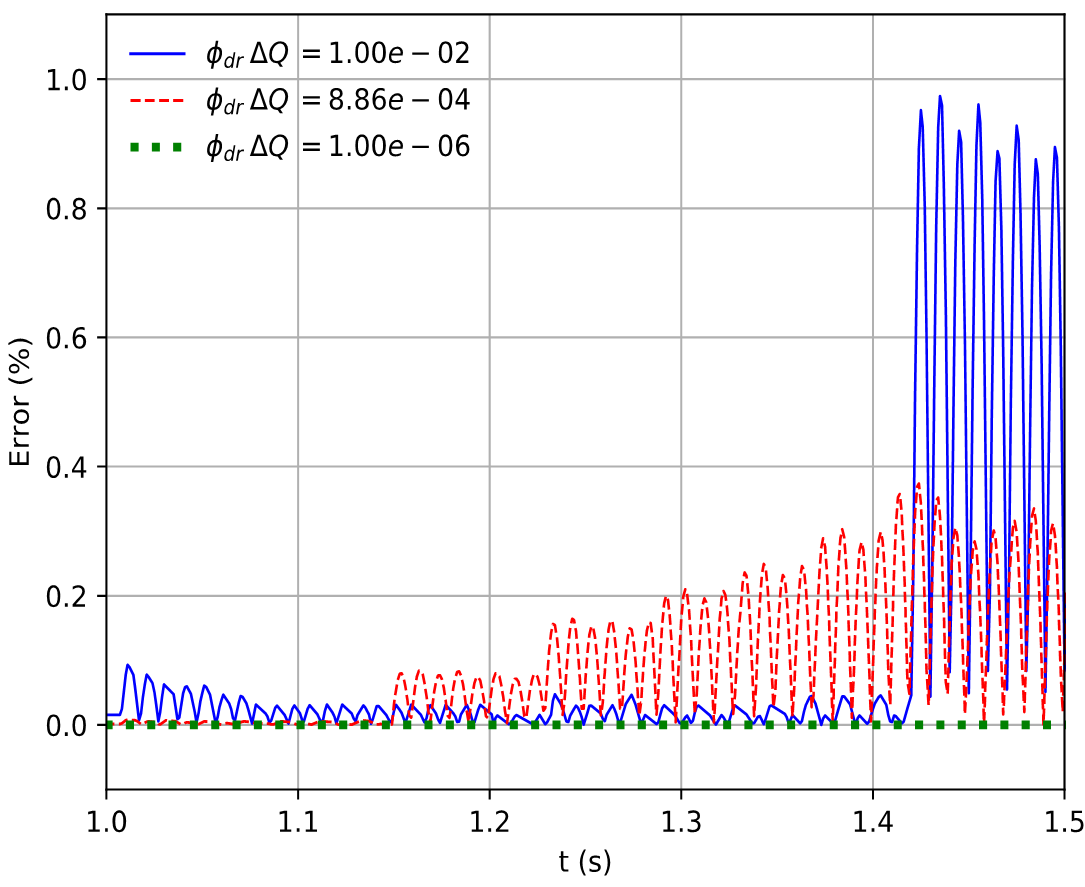
\includegraphics[width=0.8\linewidth]{syncmach_wr_error_time.png}
    \caption{Error between reference solution and QDL solution of rotor d-axis flux for several different quantization sizes $\Delta Q = 10^{-2}$ , $\Delta Q = 8.86\cdot 10^{-4}$, $\Delta Q = 10^{-6}$.}
    \label{fig:syncmach_wr_error_time}
\end{figure} 

To generate the data shown in figure \ref{fig:syncmach_wr_error_qstep} we quantized the rotor speed at $\Delta Q = 10^{-7}$ and the other state variables at $\Delta Q = 10^{-4}$. This was an experiment to see if choosing a relatively small quantization size for some particular interesting state, but leaving other quanta larger, would produce fewer updates for the whole system, while still having a small error for the particular state of interest. Figure \ref{fig:syncmach_wr_error_qstep} shows that the state of rotor speed experienced a high number of updates, but the error did not reduce compared to the simulation with system-wide $\Delta Q = 10^{-4}$, which produced the same output with a smaller number of updates. 

\begin{figure}[h]
    \centering
    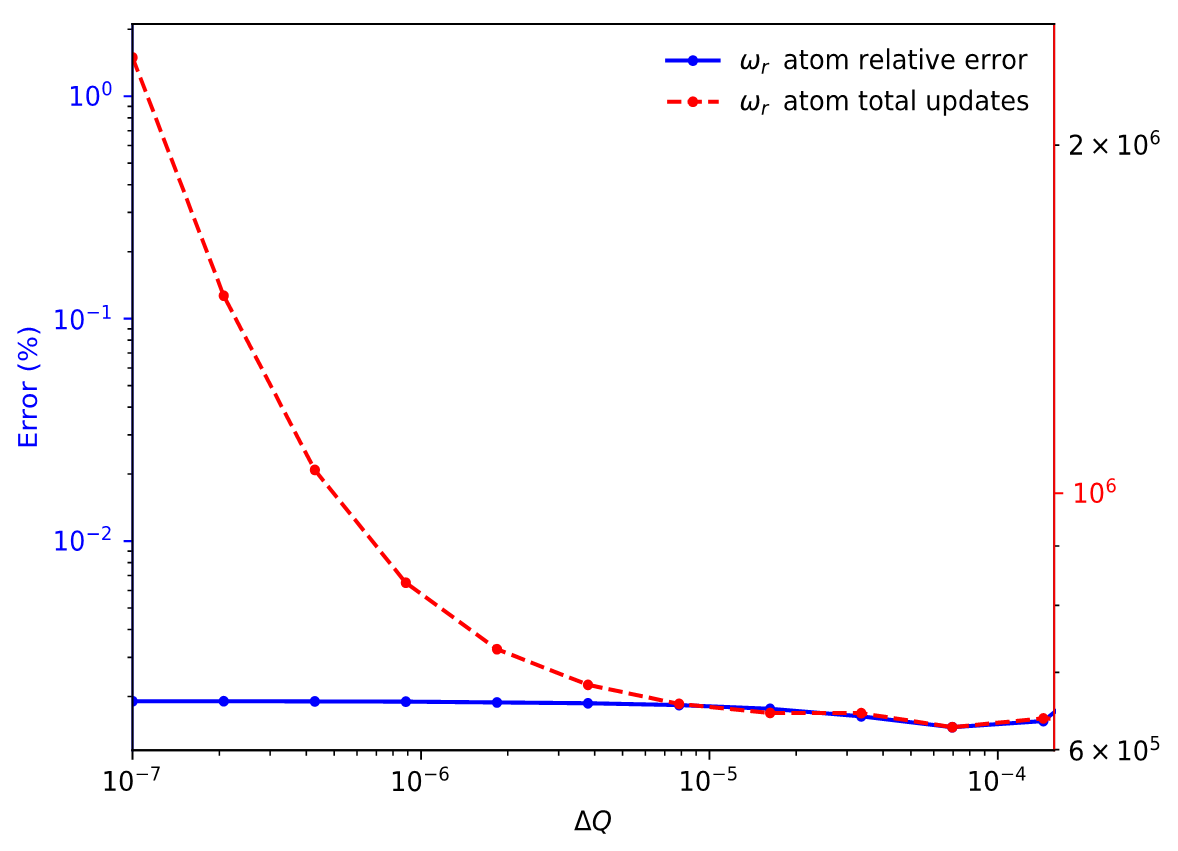
\includegraphics[width=0.8\linewidth]{syncmach_wr_error_qstep.png}
    \caption{Rotor speed updates vs relative error when rotor speed $\Delta Q$ is set to $10^{-7}$  and the quantization size of the rest of the system variables is $\Delta Q = 10^{-4}$. Possibly unnecessary high precision with low benefit of error reduction}
    \label{fig:syncmach_wr_error_qstep}
\end{figure} 

Figure \ref{fig:syncmach_error_qstep_all} shows the maximum error among any system variable at any time during the simulation interval. The graph is plotted on a logarithmic scale as a function of the $\Delta Q$, which was varied from $10^{-6}$ to $10^{-2}$ Wb. Also plotted is the corresponding sum of all updates of all atoms over the entire simulation. For small $\Delta Q$ values of $10^{-6}$ to $10^{-5}$ Wb, the error is very small and largely independent of $\Delta Q$. A logarithmic scale is used to emphasize that for very small $\Delta Q$ values ($10^{-5}$ Wb), a decrease in $\Delta Q$ does not improve the accuracy, but it does impose a penalty on computational intensity (simulation update rate), and the simulation takes longer to advance through time with no- significant error reduction. A sweet spot is evident around $\Delta Q$ between $10^{-5}$  to $10^{-4}$, where computational intensity has become relatively low while error also remains low. Above $\Delta Q$ values of around $10^{-4}$, the error increases rapidly, but without a consistent reductions in computational intensity.

\begin{figure}[h]
    \centering
    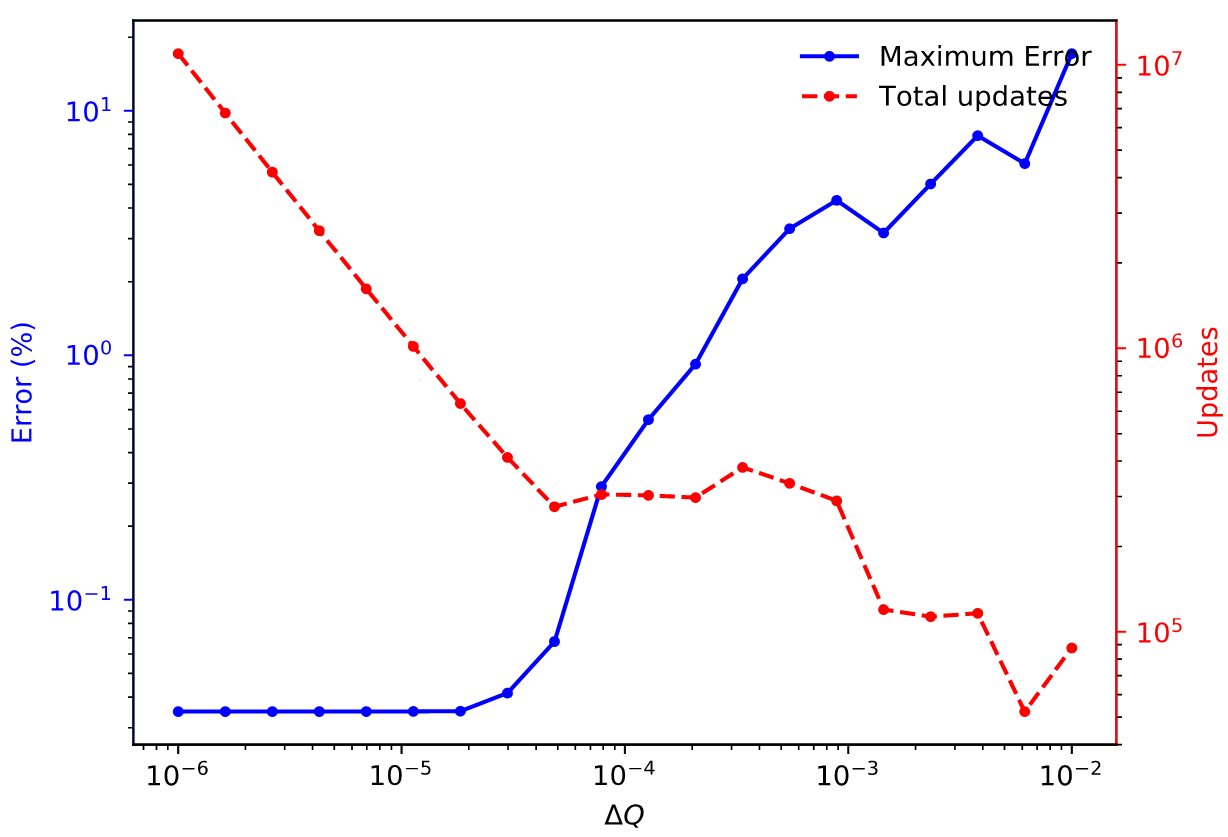
\includegraphics[width=0.8\linewidth]{syncmach_error_qstep_all.png}
    \caption{Maximum Error of all atoms for different $\Delta Q$ values. Total number of the updates decreases as the system is simulated with bigger $\Delta Q$ values at the expense of increasing the error.}
    \label{fig:syncmach_error_qstep_all}
\end{figure} 

Although the QDL method does accurately track the reference solution, the method does inherently exhibit steady-state oscillations. These oscillations are evident in figure \ref{fig:syncmach_fdr_ripple}, which shows the direct axis rotor flux at high resolution just near the onset of the torque ramp at 15 seconds. The amplitudes of these high frequency oscillations reduce as the $\Delta Q$ is reduced, but the oscillations are always present. Each oscillation represents an update event, so reducing the oscillation size comes at the expense of computation time. Figures \ref{fig:syncmach_fdr_ripple} and \ref{fig:syncmach_fdr_transient} show these high frequency oscillations at $\Delta Q$ values of $10^{-4}$  and $10^{-5}$. The mitigation of this high-frequency oscillation behavior is discussed further in chapter \ref{chap:steadystate}. 

\begin{figure}[h]
    \centering
    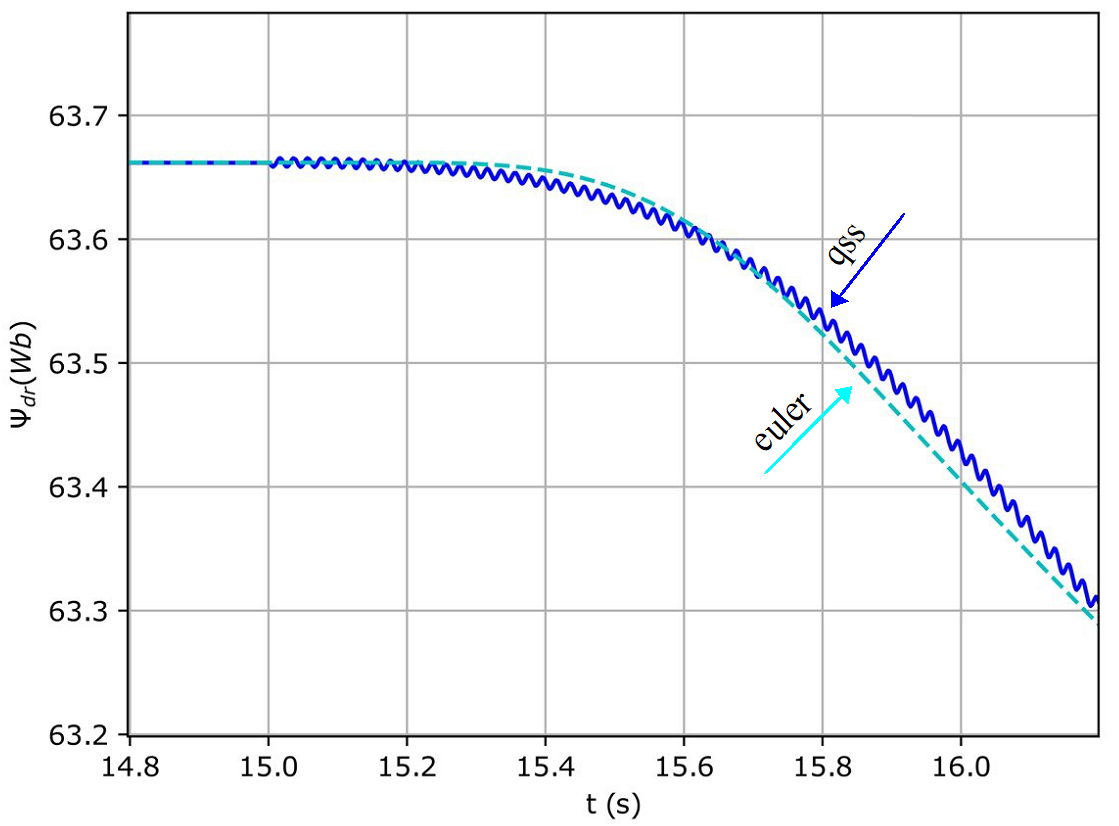
\includegraphics[width=0.8\linewidth]{syncmach_fdr_ripple.png}
    \caption{High resolution plot showing the ripples in QDL solution of the rotor d-axis flux $\psi_{dr}$ with $\Delta Q$ of $10^{-4}$.}
    \label{fig:syncmach_fdr_ripple}
\end{figure}

\begin{figure}[h]
    \centering
    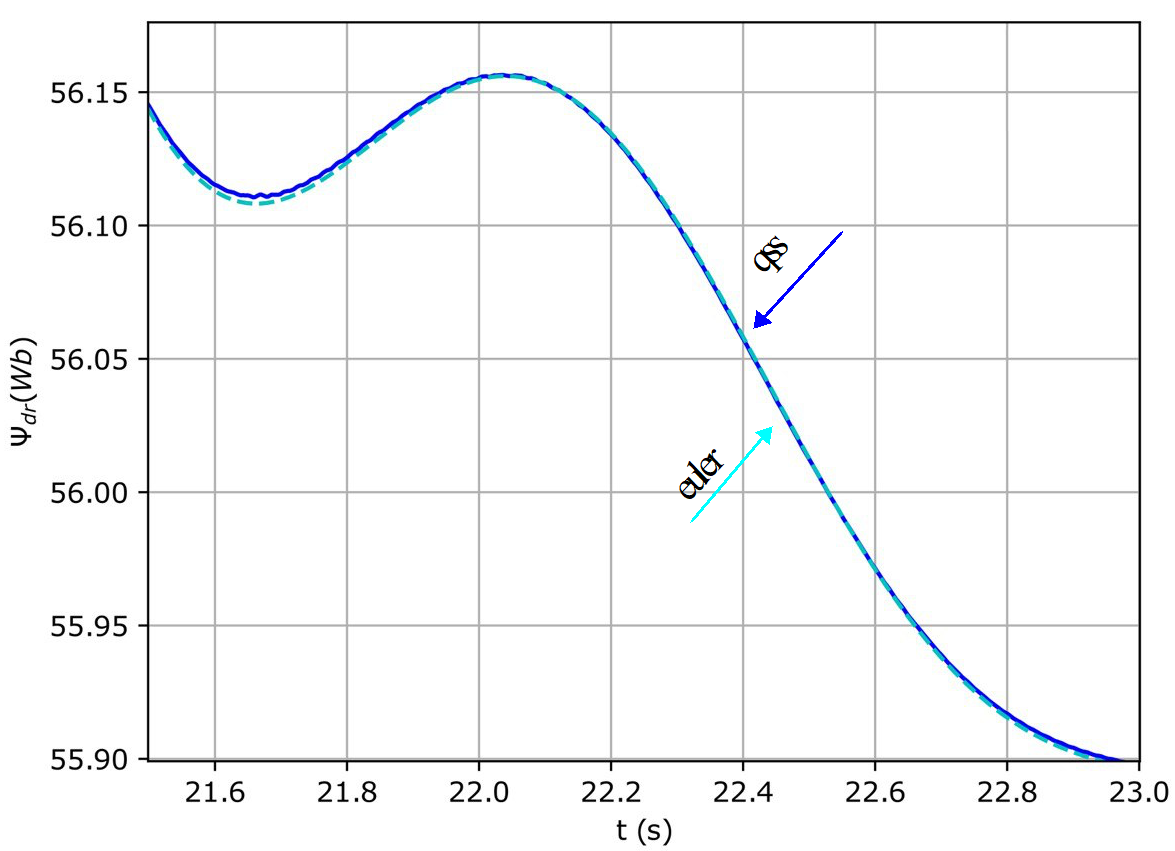
\includegraphics[width=0.8\linewidth]{syncmach_fdr_transient.png}
    \caption{High resolution plot showing the ripples in the QDL solution of the rotor d-axis flux $\psi_{dr}$ with $\Delta Q$ of $10^{-5}$. The amplitude of the ripples is smaller compared to $\Delta Q$ of $10^{-4}$.}
    \label{fig:syncmach_fdr_transient}
\end{figure}

\section{Study Summary}

The performance of the QDL method for analyzing the dynamics of non-linear power system that includes a detailed synchronous machine model has been investigated. Uniform quantization of system state variables at 0.01 percent was found to yield accuracy within 0.4 percent of that achieved with a conventional implicit state-space solution, but with a significant advantage in computational intensity, especially for systems that operate for long times in a quasi-steady-state. Since the QDL method enables the user to individually set the quantization step size ($\Delta Q$) values of each state, we evaluated performance as a function of $\Delta Q$. When the system was simulated using one uniform quantization size for all states, the total number of state updates generally decreased as $\Delta Q$ increased, but above a quantization size of about $10^{-4}$, further increase in $\Delta Q$ did not significantly reduce the computational cost (but it did decrease the simulation accuracy). When $\Delta Q$ for a single state of interest was set smaller than the uniform $\Delta Q$ of other states, refining the $\Delta Q$ of that particular state variable did not necessarily improve the error of that particular state, but it did logarithmically increase the state update intensity of the whole system. The observations of the effects of $\Delta Q$ selection are limited by the particular system that was studied. Other systems, especially those having state variables that are widely different in magnitude, may behave differently.
